\documentclass[a4paper]{report}

% Review all biblio is referenced
% Review all figures are referenced

\usepackage{graphicx}
\usepackage{float}
\usepackage{hyperref}
\usepackage{xcolor}
\usepackage[spanish]{babel}
\usepackage{listings}
\usepackage{enumitem}
\usepackage[utf8]{inputenc}

\lstset{language=c, frame=tlrb, basicstyle=\scriptsize, breaklines=true, numberbychapter=false,numbers=left}
\setlist[enumerate]{noitemsep}
\setlist[itemize]{noitemsep}

\bibliographystyle{unsrt}

\begin{document}

\renewcommand{\tablename}{Tabla}

\title{Universidad Nacional de La Plata\\Facultad de Informática\\ \bigskip
  Especialización en Cómputo de Altas Prestaciones y Tecnología Grid\\ \bigskip
  Herramientas para el Soporte de Análisis de Rendimiento}

\author{
  Alumno: Andrés More - {\tt amore@hal.famaf.unc.edu.ar}\\
  Director: Dr Fernando G. Tinetti - {\tt fernando@lidi.info.unlp.edu.ar}
}

\date{Agosto de 2013}

\maketitle

\begin{abstract}

 Este documento describe una investigación realizada como trabajo final para la Especialización en Cómputo de Altas Prestaciones dictada en la Facultad de Informática de la Universidad Nacional de La Plata. El tema de investigación consiste en métodos y herramientas para el análisis del comportamiento de aplicaciones de alto rendimiento.

  \bigskip

  Este trabajo contribuye con un resumen de la teoría de análisis de rendimiento más una descripción de las herramientas de soporte 
  disponibles en el momento. Se propone también un proceso para analizar el rendimiento, ejemplificando su aplicación a un conjunto de núcleos de
  cómputo no triviales.

\bigskip

  Luego de la introducción de terminología y bases teóricas del análisis cuantitativo de rendimiento, se detalla la experiencia de utilizar herramientas para conocer dónde se deberían localizar los esfuerzos de optimización.  Este trabajo resume la experiencia que debe atravesar cualquier investigador en busca de las diferentes alternativas para el análisis de rendimiento; incluyendo la selección de herramientas de soporte y la definición de un procedimiento sistemático de optimización.

  \bigskip

\end{abstract}

\tableofcontents

\chapter{Introducción}\label{chap:intro}

Este capítulo introduce este trabajo y su alcance. Luego de revisar la motivación de esta investigación y su alcance, se resume el estado actual del análisis
del rendimiento y se detalla el contenido restante del informe.

\section{Motivación}

En el área de cómputo de altas prestaciones los desarrolladores son los mismos
especialistas del dominio del problema a resolver. Las rutinas
más demandantes de cálculo son en su mayoría científicas y su
alta complejidad hace posible su correcta implementación sólo por los mismos investigadores.
Estas cuestiones resultan en un tiempo reducido de análisis de resultados
e impactan directamente en la productividad de los grupos de investigación y
desarrollo.

\bigskip

Con mayor impacto que en otras áreas de la computación, el código
optimizado correctamente puede ejecutarse órdenes de magnitud mejor que una implementación
directa \cite{mm-tool}. Además, se utiliza
programación en paralelo para obtener una mejor utilización de la
capacidad de cómputo disponible; aumentando por lo tanto la complejidad de
implementación, depuración y optimización \cite{is-parallel-programming-hard}.

\bigskip

Frecuentemente el proceso de optimización termina siendo
hecho de modo {\it ad-hoc}, sin conocimiento pleno de las herramientas disponibles y
sus capacidades, y sin la utilización de información cuantitativa para dirigir los
esfuerzos de optimización. Es incluso frecuente la implementación directa
de algoritmos en lugar de la utilización de librerías ya disponibles, optimizadas
profundamente y con correctitud comprobada.

\section{Alcance}

Este trabajo considera en particular a los sistemas de memoria distribuida corriendo sobre
{\it software} libre GNU/Linux, inicialmente denominados sistemas Beowulf \cite{beowulf-parallel-workstation}. A través de las
estadísticas mostradas por el Top500 \footnote{El Top500 es una lista actualizada de super-computadoras
de acuerdo al benchmark {\it Linpack}, disponible en {\tt http://www.top500.org}.}, se
puede determinar que son los más utilizados en el cómputo de aplicaciones de alto rendimiento en la actualidad.

\section{Estado Actual}

Actualmente existen numerosas y diversas herramientas para el análisis de rendimiento \cite{gregg}.
Estas funcionan a diferentes niveles de abstracción: desde contadores de eventos
a nivel de {\it hardware}, pasando por monitores de recursos dentro del núcleo del sistema operativo, instrumentación de código, y hasta la simple utilización del tiempo de ejecución de una aplicación o la comparación contra un trabajo similar de referencia.
Para poder analizar del rendimiento un desarrollador aplica las herramientas listadas en la tabla \ref{table:tools}.

\begin{table}[H]
    \caption{Herramientas de Soporte para Optimización}
    \centering
    \begin{tabular}{|l|l|}\hline
      {\bf Herramienta} & {\bf Descripción} \\ \hline
      {\tt gprof} & Muestra información de perfil de llamadas a funciones \\ \hline
      {\tt perf} & Muestra información de perfil de sistema \\ \hline
      {\it STREAM} & Benchmark de jerarquía de memoria \\ \hline
      HPL & Benchmark de capacidad de cómputo \\ \hline
      IMB Ping Pong & Benchmark de latencia y ancho de banda de red \\ \hline
      HPCC & Paquete de benchmarks \\ \hline
    \end{tabular}
    \label{table:tools}
\end{table}

Las pruebas de rendimiento como STREAM, HPL, IMB Ping Pong y HPCC permiten conocer el estado del sistema y los límites de rendimiento en la práctica.
Los perfiles de ejecución de aplicaciones y sistema permiten conocer como se utilizan los recursos del sistema para llevar a cabo las instrucciones de cada programa.

\section{Organización del Contenido}

El siguiente capítulo discute el análisis de rendimiento, sus
principios y teoría básica. El capítulo \ref{chapter:tools} detalla las herramientas más
utilizadas. El capítulo \ref{chapter:procedure} aplica las herramientas revisadas a través de un proceso sistemático. El capítulo \ref{chapter:cases} ejemplifica la aplicación del proceso con algunos núcleos de computo. El capítulo \ref{chapter:conclusions} concluye y detalla posibles extensiones de este trabajo.

\chapter{Análisis de Rendimiento}\label{chapter:analysis}

Este capítulo introduce el concepto de rendimiento y teoría básica sobre su análisis.
Además ejemplifica las actividades a realizar durante el análisis.

\section{Definición}

El rendimiento se caracteriza por la cantidad de trabajo de cómputo que se
logra en comparación con la cantidad de tiempo y los recursos ocupados.
El rendimiento debe ser evaluado entonces de forma cuantificable, utilizando alguna
métrica en particular de modo de poder comparar relativamente dos sistemas o
el comportamiento de un mismo sistema bajo una configuración distinta.

\section{Paralelismo}

Una vez obtenida una implementación eficiente, la única alternativa para mejorar el rendimiento es explotar el paralelismo que
ofrecen los sistemas de cómputo. Este paralelismo se puede explotar a diferentes niveles, desde instrucciones especiales que ejecutan sobre varios
datos a la vez (vectorización), hasta la utilización de múltiples sistemas para distribuir el trabajo.

\bigskip

 El cálculo de las mejoras posibles de rendimiento, cómo priorizarlas y la estimación de su límite máximo es una tarea compleja. Para ello existen algunas leyes fundamentales utilizadas durante el análisis de rendimiento.

\subsection{Ley de {\it Amdahl}}

 La ley de {\it Amdahl} \cite{amdahl} dimensiona la mejora que puede obtenerse en un sistema de acuerdo a las mejoras logradas en sus componentes. Nos ayuda a establecer un límite máximo de mejora y a estimar cuales pueden ser los resultados de una optimización.

\bigskip

La mejora de un programa utilizando cómputo paralelo está limitado por el tiempo necesario para completar su fracción serial o secuencial. En la mayoría de los casos, el paralelismo sólo impacta notoriamente cuando es utilizado en un pequeño número de procesadores, o cuando se aplica a problemas altamente escalables ({\it Embarrassingly Parallel Problems}). Una vez paralelizado un programa, los esfuerzos suelen ser enfocados en cómo minimizar la parte secuencial, algunas veces haciendo más trabajo redundante pero en forma paralela.

\bigskip

Suponiendo que una aplicación requiere de un trabajo serial más un trabajo paralelizable, la ley de {\it Amdahl} calcula la ganancia ($ S $) mediante la Ecuación \ref{eq:amdahl}.
Donde $ P $ es el porcentaje de trabajo hecho en paralelo, ($ 1-P $) es entonces el trabajo en serie o secuencial, y $ N $ la cantidad de unidades de cómputo a utilizar.

\begin{eqnarray}
\label{eq:amdahl}
S = \frac{1}{(1 - P) + \frac{P}{N}}
\end{eqnarray}

Esta ley nos establece que incluso teniendo infinitas unidades de cómputo la ganancia está limitada.
La Tabla \ref{fig:amdahl} muestra que no importa la cantidad de unidades de
procesamiento que sean utilizadas.

\begin{table}[H]
\caption{Mejora Máxima}
\centering
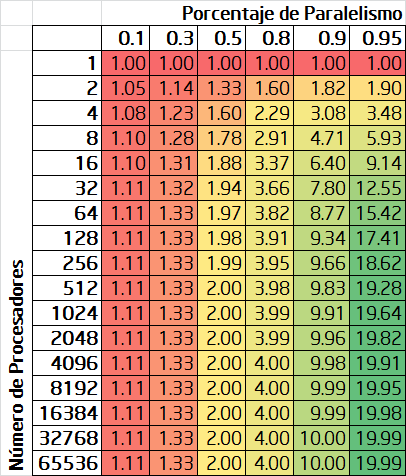
\includegraphics[width=7cm]{amdahl.png}

\label{fig:amdahl}
\end{table}

Por ejemplo, en el caso de tener solo un $ 10\% $ de paralelismo
en una aplicación, la mejora nunca va a superar $ 1.10x $ la original.
En el caso de tener un $ 95\% $, la mejora no puede ser mayor a $ 20x $.

\subsection{Ley de {\it Gustafson}}

Desde un punto de vista más general, la ley de {\it Gustafson}
\cite{gustafson} (computada mediante la Ecuación \ref{eq:gustafson})
establece que las aplicaciones que manejan problemas
repetitivos con conjuntos de datos similares pueden ser fácilmente
paralelizadas. En comparación, la ley anterior no escala el tamaño o
resolución de problema cuando se incrementa la potencia de cálculo, es
decir asume un tamaño de problema fijo. 

\begin{eqnarray}
\label{eq:gustafson}
speedup(P) = P - \alpha \times ( P - 1)
\end{eqnarray}

donde $ P $ es el número de unidades de cómputo y $ \alpha $ el porcentaje de trabajo paralelizable.

\bigskip

Al aplicar esta ley obtenemos que un problema con datos grandes o repetitivos en cantidades grandes puede ser computado en paralelo muy eficientemente. Nos es útil para determinar el tamaño de problema a utilizar cuando los recursos de cómputo son incrementados. En el mismo tiempo de ejecución, el programa resuelve entonces problemas más grandes.

\begin{table}[H]
\caption{Tamaño de Datos de Entrada}
\centering
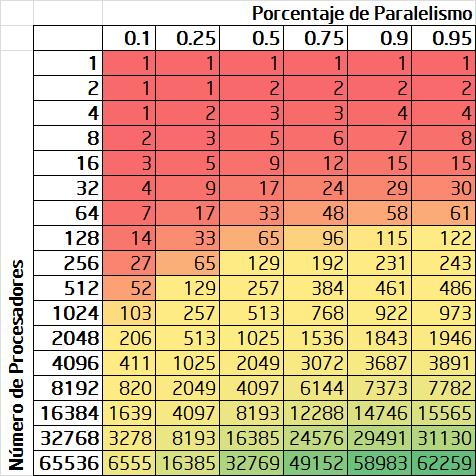
\includegraphics[width=7cm]{gustafson.png}
\label{fig:gustafson}
\end{table}

Similarmente al cuadro anterior, podemos deducir de la Tabla \ref{fig:gustafson} que en el caso de un programa con sólo $ 10\% $ de paralelismo, al incrementar los recursos 64x sólo podemos incrementar el tamaño del problema $ 7x $. Sin embargo nos calcula
un incremento de $ 61x $ en el caso de tener $ 95\% $ de paralelismo.

\subsection{Métrica de {\it Karp-Flatt}}

Esta métrica es utilizada para medir el grado de paralelismo de una aplicación \cite{karp-flatt}. Esta métrica nos permite rápidamente estimar la mejora posible al aplicar un alto nivel de paralelismo.

\bigskip

Dado un cómputo paralelo con una mejora de rendimiento $ \psi $ en $ P $
procesadores, donde $ P > 1 $. La fracción serial {\it Karp-Flatt} representada con $ e $ y calculada según la Ecuación \ref{eq:karp-flatt} es determinada experimentalmente, mientras menor sea $ e $ mayor se supone el nivel de paralelismo posible.

\begin{eqnarray}
\label{eq:karp-flatt}
 e = \frac{\frac{1}{\psi} - \frac{1}{p}}{1 - \frac{1}{p}} 
\end{eqnarray}

Para un problema de tamaño fijo, la eficiencia típicamente disminuye cuando
el número de procesadores aumenta. Se puede entonces determinar si esta disminución
es debida a un paralelismo limitado, a un algoritmo no optimizado o un problema de
arquitectura del sistema.

\section{Métricas}

Algunos ejemplos de medida de rendimiento son:

\begin{enumerate}
\item El ancho de banda y la latencia mínima de un canal de comunicación,
  una jerarquía de memorias o de la unidad de almacenamiento.
\item La cantidad de instrucciones, operaciones, datos o trabajo procesado
  por cierta unidad de tiempo.
\item El rendimiento asociado al costo del equipamiento, incluyendo mantenimiento
 periódico, personal dedicado y gastos propios del uso cotidiano.
\item El rendimiento por unidad de energía consumida (electricidad).

\end{enumerate}

Un método de medición de rendimiento indirecto consiste en medir el uso de
los recursos del sistema mientras se ejercita el mismo con un trabajo dado.
Por ejemplo: el nivel de carga de trabajo en el sistema, la cantidad de operaciones realizadas por el
sistema operativo o la unidad de procesamiento, la utilización de memoria o
archivos temporales e incluso el ancho de banda de red utilizado durante la comunicación.

\section{Técnicas de Análisis}

El procedimiento de mejora general usualmente consiste en ciclos iterativos de medir, localizar, optimizar y
comparar (Figura \ref{fig:cycle}). Es muy importante mantener la disciplina en realizar un cambio a la
vez ya que esto asegura resultados reproducibles y convergentes, sin efectos no deseados.

\begin{figure}[H]
\begin{center}
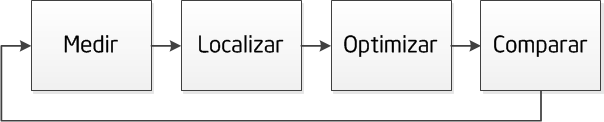
\includegraphics[width=10cm]{cycle.png}
\caption{Optimización Iterativa}
\label{fig:cycle}
\end{center}
\end{figure}

A la hora de tomar decisiones, éstas deben estar basadas en datos concretos, ya que en caso contrario se podría estar trabajando sin llegar a obtener un rédito adecuado.

\bigskip

En el caso de tener problemas de desviación en los resultados medidos, es aconsejable obtener un gran número de muestras y utilizar un valor promedio para asegurarse de evitar errores de medición tanto como sea posible. También es preferible aumentar el tamaño del problema a resolver, o la definición de los resultados para ejercitar por más tiempo y tener así un resultado más estable.
Suponiendo una distribución normal de resultados, se suelen controlar que haya menos de 3 $ \sigma $ de diferencia. Se busca que la mayoría de los resultados queden cerca de su promedio, como muestra la Figura \ref{fig:deviation}.

\begin{figure}[H]
\centering
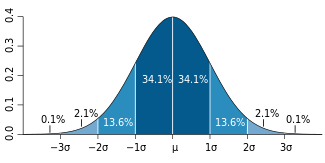
\includegraphics[width=8cm]{deviation.png}
\caption{Desviación de valores en una distribución normal [Wikipedia]}
\label{fig:deviation}
\end{figure}

Los resultados deben también ser correctamente guardados para evitar
problemas de datos. Si la configuración del sistema es dinámica entonces la
reproducción de resultados es no trivial. En el caso de no tener una
configuración de sistema estable en el tiempo, es recomendable siempre
ejecutar una versión optimizada contra una versión de referencia en un mismo
sistema de cómputo.

\bigskip

Para comparar es recomendable utilizar la media geométrica según la Ecuación \ref{eq:geomean} en lugar de la aritmética \cite{how-not-to-lie}, ya que permite dimensionar la tendencia central de un valor típico en un conjunto de números. Esto permite reducir el impacto de ruido introducido por una ejecución problemática.

\begin{equation}
\label{eq:geomean}
G = \sqrt[n]{x_{1} \ldots x_{n}}
\end{equation}

La raíz n-ésima de un número (para un $ n $ posiblemente muy grande), es una operación ineficiente ya que se implementa con métodos numéricos de aproximación siguiendo el método de {\it Newton} \cite{numerical-analysis}. En cambio se suele tomar el anti-logaritmo del promedio de los logaritmos de los valores siguiendo la ecuación \ref{eq:geomean-log}.

\begin{equation}
\label{eq:geomean-log}
G = 10 ^{( log _{10} (x_{1}) + \ldots + log _{10} (x_{n}) ) / n}
\end{equation}

\chapter{Herramientas de Soporte}\label{chapter:tools}

Este capítulo revisa las herramientas disponibles para soporte de análisis
de rendimiento de aplicaciones.

\section{Pruebas de Rendimiento}

Para medir el rendimiento se utilizan pruebas de referencia ({\em benchmarks}); éstas pueden ser aplicaciones sintéticas construidas específicamente, o bien aplicaciones del mundo real computando un problema prefijado. Al tener valores de referencia se pueden caracterizar los sistemas de modo de predecir el rendimiento de una aplicación.
Los valores a los que se llegan con un {\it benchmark} suelen ser más prácticos y
comparables que los teóricos de acuerdo a condiciones ideales de uso de recursos.
También es posible garantizar que el sistema sigue en un mismo estado con el correr
del tiempo y después de cambios de configuraciones en {\it hardware} o {\it software}.

\bigskip

Las características deseables en un {\it benchmark} son portabilidad, simplicidad, estabilidad y
reproducción de resultados. Esto permite que sean utilizadas para realizar
mediciones cuantitativas y así realizar comparaciones de optimizaciones o
entre sistemas de cómputo diferentes. También se pide que el tiempo de
ejecución sea razonable y que el tamaño del problema sea ajustable para
poder mantener su utilidad con el paso del tiempo y el avance de las
tecnologías.

\bigskip

A continuación se introducen algunas de las más utilizadas para cómputo
de altas prestaciones (listadas en la tabla \ref{table:benchmark-list}),
y posteriormente algunos detalles específicos e instancias
de sus datos de salida para ser utilizados a manera de ejemplo.

\begin{table}[H]
    \caption{Benchmarks}
    \centering
    \begin{tabular}{|l|l|l|}\hline
      {\bf Benchmark} & {\bf Componente} & {\bf Descripción} \\ \hline
      STREAM & Memoria & Ancho de banda sostenido \\ \hline
      Linpack & Procesador & Operaciones de punto flotante \\ \hline
      IMB Ping Pong & Red & Latencia/Ancho de banda de red \\ \hline
      HPCC & Sistema & Múltiples componentes \\ \hline
        \end{tabular}
  \label{table:benchmark-list}
\end{table}

\bigskip

Los {\it benchmarks} pueden ser utilizados para diferentes propósitos. Primero,
los valores reportados son usados como referencia para contrastar rendimiento.
Segundo, su desviación demuestra que algo ha cambiado en el sistema (por lo tanto
su no desviación indica que el sistema sigue saludable). Por último,
un {\it benchmark} sintético implementando el cómputo que uno quiere realizar
muestra el rendimiento máximo posible a obtener en la práctica.

\subsection{STREAM}

STREAM \cite{stream} es un {\it benchmark} sintético que mide el ancho de banda de memoria sostenido en MB/s y el rendimiento de computación relativa de algunos vectores simples de cálculo. Se utiliza para dimensionar el ancho de banda de acceso de escritura o lectura a la jerarquía de memoria principal del sistema bajo análisis. Dentro de una misma ejecución de este {\it benchmark} se ejercitan diferentes operaciones en memoria, listadas en la tabla \ref{table:stream}.

\begin{table}[H]
\caption{Operaciones del Benchmark STREAM}
  \centering
    \begin{tabular}{|l|l|l|}\hline
      {\bf Función} & {\bf Operación} & {\bf Descripción} \\ \hline
      copy & $ \forall i $ $ b_{i} = a_{i} $ & Copia simple \\ \hline
      scale & $ \forall i $ $ b_{i} = c \times a_{i} $ & Multiplicación escalar \\ \hline
      add & $ \forall i $ $ c_{i} = b_{i} + a_{i} $ & Suma directa \\ \hline
      triad & $ \forall i $ $ c_{i} = b_{i} + c \times a_{i} $ & Suma y multiplicación escalar \\ \hline
    \end{tabular} 
 \label{table:stream}
\end{table}

La salida en pantalla muestra entonces los diferentes tiempos conseguidos y la cantidad de información transferida por unidad de tiempo.
Como último paso, el programa valida también la solución computada.

{\small
\begin{verbatim}
  STREAM version $Revision: 1.2 $
  -------------------------------------------------------------
  This system uses 8 bytes per DOUBLE PRECISION word.
  -------------------------------------------------------------
  Array size = 10000000, Offset = 0
  Total memory required = 228.9 MB.
  Each test is run 10 times, but only the *best* time is used.
  -------------------------------------------------------------
  Function     Rate (MB/s)   Avg time     Min time     Max time
  Copy:        4764.1905       0.0337       0.0336       0.0340
  Scale:       4760.2029       0.0338       0.0336       0.0340
  Add:         4993.8631       0.0488       0.0481       0.0503
  Triad:       5051.5778       0.0488       0.0475       0.0500
  -------------------------------------------------------------
  Solution Validates
\end{verbatim}
}

\subsection{Linpack}

Linpack \cite{linpack} es un conjunto de subrutinas {\it FORTRAN} que resuelven
problemas de álgebra lineal como ecuaciones lineales y multiplicación de
matrices. High Performance Linpack (HPL) \cite{hpl} es una versión portable del {\it benchmark} que incluye
el paquete Linpack pero modificado para sistemas de memoria distribuida.

\bigskip

Este {\it benchmark} es utilizado mundialmente para la comparación de la
velocidad de las supercomputadoras en el ranking TOP500. 
Un gráfico del TOP500 de los últimos años (Figura \ref{fig:top500}) demuestra claramente la
tendencia en crecimiento de rendimiento; también la relación entre el primero,
el último y la suma de todos los sistemas en la lista.

\begin{figure}[H]
\centering
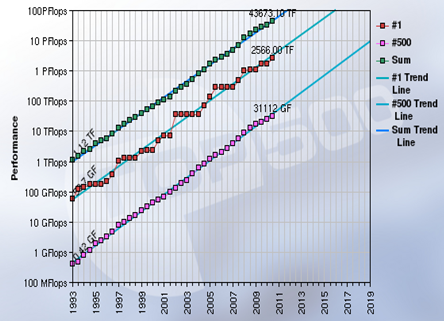
\includegraphics[width=12cm]{top500.png}
\caption{Rendimiento Agregado del Top500 [Top500])}
\label{fig:top500}
\end{figure}

Este {\it benchmark} requiere conocimiento avanzado para una correcta configuración,
por ejemplo el tamaño de bloque que se va a utilizar para la distribución de trabajo
debe estar directamente relacionado con el tamaño del {\it cache} de memoria del procesador.

\bigskip

La salida en pantalla resume entonces los datos de entrada y los resultados conseguidos.
Como último paso el programa valida que los resultados sean correctos.

{\small
\begin{verbatim}
=================================================================
HPLinpack 2.0 - High-Performance Linpack benchmark - Sep 10, 2008
Written by A. Petitet and R. Clint Whaley
=================================================================
The following parameter values will be used:
N      :   28888
NB     :     168
PMAP   : Row-major process mapping
P      :       4
Q      :       4
PFACT  :   Right
NBMIN  :       4
NDIV   :       2
RFACT  :   Crout
BCAST  :  1ringM
DEPTH  :       0
SWAP   : Mix (threshold = 64)
L1     : transposed form
U      : transposed form
EQUIL  : yes
ALIGN  : 8 double precision words
------------------------------------------------------------------
- The matrix A is randomly generated for each test.
- The relative machine precision (eps) is taken to be 1.110223e-16
- Computational tests pass if scaled residuals are less than 16.0

Column=000168 Fraction=0.005 Mflops=133122.97
...
Column=025872 Fraction=0.895 Mflops=98107.60
======================================================================
T/V                N   NB   P    Q             Time             Gflops
WR01C2R4       28888  168   4    4           165.83          9.693e+01
----------------------------------------------------------------------
||Ax-b||_oo/(eps*(||A||_oo*||x||_oo+||b||_oo)*N) = 0.0043035 .. PASSED
======================================================================
Finished      1 tests with the following results:
1 tests completed and passed residual checks,
0 tests completed and failed residual checks,
0 tests skipped because of illegal input values.
\end{verbatim}
}

\bigskip

Existe cierta controversia de que no es una buena forma de ejercitar un
sistema de cómputo distribuido ya que no implica uso significativo de la
red, sólo procesamiento intensivo de aritmética de punto flotante
sobre la jerarquía local de memoria.

\subsection{Intel MPI Benchmarks}

Es un conjunto de {\it benchmarks} cuyo objetivo es ejercitar las funciones
más importantes del estándar para librerías de paso de mensajes (MPI, por sus siglas en inglés) \cite{mpi-standard}.
El más conocido es el popular ping-pong, el cual ejercita la transmisión de mensajes ida y vuelta entre dos nodos de
cómputo con diferentes tamaños de mensajes. \cite{latency}.

\bigskip

Para obtener el máximo ancho de banda disponible, se ejercita la comunicación a través de mensajes con datos grandes. Para obtener la mínima latencia, se ejercita la comunicación con mensajes vacíos, es decir transmitiendo mensajes sin dato alguno.

{\small
\begin{verbatim}
# Intel (R) MPI Benchmark Suite V3.1, MPI-1 part
# Date                  : Wed Mar  3 10:45:16 2010
# Machine               : x86_64
# System                : Linux
# Release               : 2.6.16.46-0.12-smp
# Version               : #1 SMP Thu May 17 14:00:09 UTC 2007
# MPI Version           : 2.0
# MPI Thread Environment: MPI_THREAD_SINGLE
# Calling sequence was: ../IMB-MPI1 pingpong
# Minimum message length in bytes:   0
# Maximum message length in bytes:   4194304
#
# MPI_Datatype                   :   MPI_BYTE
# MPI_Datatype for reductions    :   MPI_FLOAT
# MPI_Op                         :   MPI_SUM
#
# List of Benchmarks to run: PingPong
#---------------------------------------------------
# Benchmarking PingPong
# #processes = 2
#---------------------------------------------------
#bytes     #repetitions  t[usec]     Mbytes/sec
0              1000           17.13        0.00
1              1000           17.89        0.05
2              1000           17.82        0.11
4              1000           17.95        0.21
...
1048576    40              8993.23    111.19
2097152    20              17919.20  111.61
4194304    10              35766.45  111.84
\end{verbatim}
}

\subsection{HPC Challenge}

El {\it benchmark} HPC Challenge \cite{hpcc} (HPCC) está compuesto internamente por un conjunto de
varios núcleos de cómputo: entre ellos STREAM, HPL, Ping Pong, Transformadas de {\it Fourier}
y otros ejercitando la red de comunicación.

\bigskip

Este benchmark muestra diferentes resultados que son representativos
y puestos en consideración de acuerdo al tipo de aplicación en discusión.
La mejor máquina depende de la aplicación específica a ejecutar, ya que algunas
aplicaciones necesitan mejor ancho de banda de memoria, mejor canal de comunicación, o
simplemente la mayor capacidad de cómputo de operaciones flotantes posible.

\bigskip

Una analogía interesante para entender cómo el {\it benchmark} se relaciona con diferentes núcleos de cómputo se muestra en la Figura \ref{fig:locality}. Por ejemplo al tener un problema que utiliza principalmente acceso a memoria local, se puede suponer que un sistema con buenos resultados de STREAM va ser útil.

\begin{figure}[H]
\begin{center}
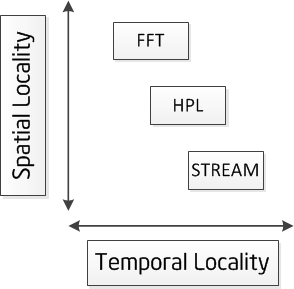
\includegraphics[width=10cm]{locality.png}
\caption{Localidad temporal versus espacial en resultados de HPCC}
\label{fig:locality}
\end{center}
\end{figure}

Para una mejor comparación de resultados de HPCC se utilizan diagramas
denominados {\it kiviats}, un ejemplo se muestra en la Figura \ref{fig:kiviat}.
Los resultados están normalizados hacia uno de los sistemas, y se puede identificar mejor rendimiento en FLOPs por poseer mejores DGEMM y HPL en comparación.

\begin{figure}[H]
\begin{center}
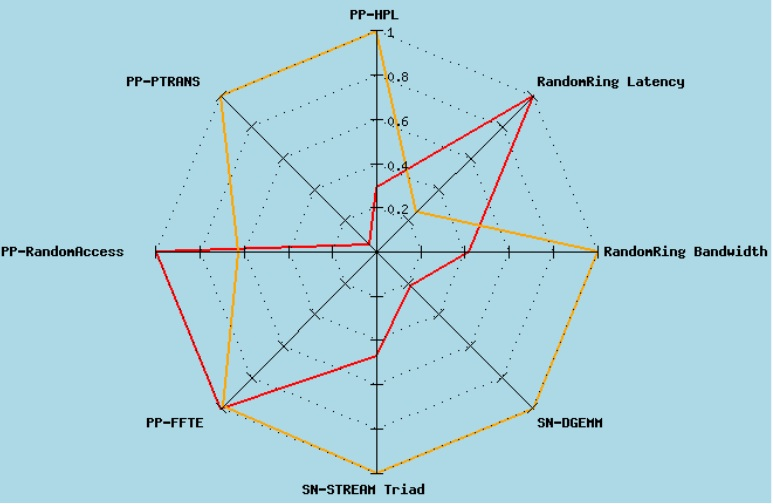
\includegraphics[width=12cm]{kiviat.png}
\caption{Diagrama Kiviat [Top500]}
\label{fig:kiviat}
\end{center}
\end{figure}

Un ejemplo de la salida que se muestra durante la ejecución se muestra a continuación.

{\scriptsize

\begin{verbatim}
This is the DARPA/DOE HPC Challenge Benchmark version 1.2.0 October 2003
Produced by Jack Dongarra and Piotr Luszczek
Innovative Computing Laboratory
University of Tennessee Knoxville and Oak Ridge National Laboratory

Begin of Summary section.
\end{verbatim}

\begin{minipage}[b]{0.5\linewidth}
\begin{verbatim}
VersionMajor=1
VersionMinor=2
LANG=C
Success=1
CommWorldProcs=3
MPI_Wtick=1.000000e-06
HPL_Tflops=0.0674008
HPL_time=26.3165
HPL_eps=1.11022e-16
HPL_N=13856
HPL_NB=64
HPL_nprow=1
HPL_npcol=3
HPL_depth=2
HPL_nbdiv=2
HPL_nbmin=8
HPL_cpfact=C
HPL_crfact=R
HPL_ctop=1
HPL_order=R
dweps=1.110223e-16
sweps=5.960464e-08
HPLMaxProcs=3
HPLMinProcs=3
DGEMM_N=4618
StarDGEMM_Gflops=68.9053
SingleDGEMM_Gflops=70.2692
PTRANS_GBs=0.794254
PTRANS_time=0.479293
PTRANS_residual=0
PTRANS_n=6928
PTRANS_nb=64
PTRANS_nprow=1
PTRANS_npcol=3
MPIRandomAccess_N=134217728
MPIRandomAccess_time=30.4475
MPIRandomAccess_Check=14.0705
MPIRandomAccess_Errors=0
\end{verbatim}
\end{minipage}
\hspace{0.1cm}
\begin{minipage}[b]{0.5\linewidth}
\begin{verbatim}
MPIRandomAccess_ErrorsFraction=0
MPIRandomAccess_ExeUpdates=536870912
MPIRandomAccess_GUPs=0.0176327
MPIRandomAccess_TimeBound=-1
MPIRandomAccess_Algorithm=0
RandomAccess_N=33554432
StarRandomAccess_GUPs=0.0186362
SingleRandomAccess_GUPs=0.0184568
STREAM_VectorSize=21332081
STREAM_Threads=8
StarSTREAM_Copy=4.34705
StarSTREAM_Scale=3.24366
StarSTREAM_Add=3.41196
StarSTREAM_Triad=3.46198
SingleSTREAM_Copy=4.53628
SingleSTREAM_Scale=3.38984
SingleSTREAM_Add=3.59073
SingleSTREAM_Triad=3.65083
FFT_N=8388608
StarFFT_Gflops=2.17339
SingleFFT_Gflops=2.26806
MPIFFT_N=8388608
MPIFFT_Gflops=1.7043
MPIFFT_maxErr=1.77722e-15
MPIFFT_Procs=2
MaxPingPongLatency_usec=5.37932
RandomRingLatency_usec=5.70686
MinPingPongBandwidth_GBytes=0.675574
NaturalRingBandwidth_GBytes=0.531278
RandomRingBandwidth_GBytes=0.529161
MinPingPongLatency_usec=5.24521
AvgPingPongLatency_usec=5.30978
MaxPingPongBandwidth_GBytes=0.682139
AvgPingPongBandwidth_GBytes=0.678212
NaturalRingLatency_usec=5.79357
FFTEnblk=16
FFTEnp=8
FFTEl2size=1048576
\end{verbatim}
\end{minipage}

\begin{verbatim}
End of Summary section.
End of HPC Challenge tests.
\end{verbatim}
}

\section{Herramientas}

Se recomienda un proceso de aplicación gradual empezando por herramientas generales de alto nivel que analizan la aplicación como un todo; terminando con herramientas de bajo nivel que proveen detalles complejos de granularidad más fina en componentes particulares del sistema. Esto permite ir analizando el rendimiento sin tener que enfrentar la dificultad de un análisis complejo y extensivo desde un principio. Una lista de las herramientas más conocidas se muestra en la Tabla \ref{table:tooling}.

\begin{table}[H]
\caption{Aplicación Gradual de Herramientas}
\begin{tabular}{|l|l|} \hline
{\bf Característica} & {\bf Herramientas} \\ \hline
Capacidad del sistema & Benchmark HPCC \\ \hline
Medición de ejecución & {\tt time}, {\tt gettimeofday()}, {\tt MPI\_WTIME()} \\ \hline
Perfil de ejecución & profilers: {\tt gprof, perf} \\ \hline
Comportamiento de la aplicación & profilers: {\tt gprof, perf} \\ \hline
Comportamiento de librerías & profilers: valgrind, MPI vampir. \\ \hline
Comportamiento del sistema & profilers: oprofile, perf \\ \hline
Vectorización & compilador: gcc \\ \hline
Contadores en {\it hardware} & oprofile, PAPI, perf \\ \hline
\end{tabular}
\label{table:tooling}
\end{table}

A grandes rasgos el procedimiento es el siguiente:

\begin{enumerate}

\item Se establece una línea de comparación al ejecutar una prueba de rendimiento del sistema, {\it HPCC} brinda un conjunto de métricas muy completo. 

\item Se utilizan herramientas para medir el tiempo de ejecución de la aplicación sobre diferentes escenarios. time permite una ejecución directa sin modificación de código, {\tt gettimeofday()} requiere modificación de código pero puede ser utilizados con mayor libertad dentro de la aplicación.  
En el caso de estar utilizando la librería MPI {\tt MPI\_WTime()} y la herramienta VAMPIR\footnote{\href{http://www.vampir.eu}{http://www.vampir.eu}} proveen soporte específico para análisis de rendimiento.

\item Se dimensiona el comportamiento de la aplicación mediante un perfil de ejecución y un análisis de cuello de botella utilizando {\tt gprof}. 

\item Se analiza el comportamiento del sistema ejecutando la aplicación mediante {\tt oprofile} \footnote{\href{http://oprofile.sourceforge.net}{http://oprofile.sourceforge.net}} o {\tt perf} \footnote{\href{https://perf.wiki.kernel.org}{https://perf.wiki.kernel.org}}. 

\item Se revisa el reporte del compilador para comprobar que se estén vectorizando los ciclos de cálculo más intensivos.

\item Se analiza el comportamiento de las unidades de cómputo utilizando soporte de {\it hardware} mediante herramientas como {\tt perf}, {\tt oprofile} y {\it Performance Application Programming Interface} (PAPI) \footnote{\href{http://icl.cs.utk.edu/papi}{http://icl.cs.utk.edu/papi}}.

\end{enumerate}

\section{Tiempo de Ejecución}

Esta sección revisa como medir el tiempo de ejecución global de una aplicación, incluyendo ejemplos.

\subsection{Tiempo de ejecución global}

Para medir el tiempo de ejecución de un comando en consola se utiliza {\tt time(1)}. Aunque rudimentaria, esta simple herramienta no necesita de instrumentación de código y se encuentra disponible en cualquier distribución {\it GNU/Linux}.
El intérprete de comandos tiene su propia versión embebida, sin embargo el del sistema brinda información del uso de otros recursos del sistema, usualmente localizado en {\tt /usr/bin/time}.

\bigskip

\begin{lstlisting}
$ /usr/bin/time -v ./script.sh
1
        Command being timed: "./script.sh"
        User time (seconds): 0.61
        System time (seconds): 0.00
        Percent of CPU this job got: 99%
        Elapsed (wall clock) time (h:mm:ss or m:ss): 0:00.62
        Average shared text size (kbytes): 0
        Average unshared data size (kbytes): 0
        Average stack size (kbytes): 0
        Average total size (kbytes): 0
        Maximum resident set size (kbytes): 4560
        Average resident set size (kbytes): 0
        Major (requiring I/O) page faults: 0
        Minor (reclaiming a frame) page faults: 668
        Voluntary context switches: 6
        Involuntary context switches: 2
        Swaps: 0
        File system inputs: 0
        File system outputs: 0
        Socket messages sent: 0
        Socket messages received: 0
        Signals delivered: 0
        Page size (bytes): 4096
        Exit status: 0
\end{lstlisting}

\subsection{Reloj del sistema}

La librería de sistema permite acceder a llamadas al sistema operativo para obtener datos precisos del paso del tiempo.
Las más utilizadas son {\tt gettimeofday(3)} y {\tt clock(3)}, aunque éste último se comporta de manera especial al utilizar multi-threading ya que suma el tiempo ejecutado en cada core.

\bigskip

El siguiente código ejemplifica como obtener un número de segundos en una representación de punto flotante de doble precisión, permitiendo una granularidad de medición adecuada.

\begin{lstlisting}
double wtime(void)
{
  double sec;
  struct timeval tv;
  
  gettimeofday(&tv, NULL);
  sec = tv.tv_sec + tv.tv_usec/1000000.0;
  return sec;
}
\end{lstlisting}

\subsection{Ejemplo: {\tt time}}

El siguiente ejemplo muestra como obtener información del uso de los recursos del sistema por parte de una aplicación.

\begin{lstlisting} 
$ /usr/bin/time -v ./program
Command being timed: "./program"
User time (seconds): 0.00
System time (seconds): 0.00
Percent of CPU this job got: 0%
Elapsed (wall clock) time (h:mm:ss or m:ss): 0:00.00
Average shared text size (kbytes): 0
Average unshared data size (kbytes): 0
Average stack size (kbytes): 0
Average total size (kbytes): 0
Maximum resident set size (kbytes): 3808
Average resident set size (kbytes): 0
Major (requiring I/O) page faults: 0
Minor (reclaiming a frame) page faults: 289
Voluntary context switches: 1
Involuntary context switches: 1
Swaps: 0
File system inputs: 0
File system outputs: 0
Socket messages sent: 0
Socket messages received: 0
Signals delivered: 0
Page size (bytes): 4096
Exit status: 0
\end{lstlisting}

\section{Perfil de Ejecución Funcional}

Estas herramientas denominadas {\it profilers} extraen el perfil dinámico de una aplicación en tiempo de ejecución. 
Se instrumenta la aplicación con una opción específica que incluye información de uso de las diferentes partes del programa y los recursos del sistema como por ejemplo procesador y memoria.

\bigskip

La aplicación debe ejecutarse con un conjunto de datos prefijado. El conjunto de
datos debe ser representativo y debe también ejercitar la aplicación por
una cantidad de tiempo suficiente como para intensificar el uso de los
recursos. Los datos del perfil de una ejecución son luego obtenidos en la
forma de un archivo de datos, luego se procede a procesar los datos acumulados
con un analizador respectivo.

\bigskip

Provee un perfil plano que consiste en una simple lista de las funciones
ejecutadas ordenadas por la cantidad acumulada de tiempo utilizado.
También provee el gráfico de llamadas anidadas, que muestra el tiempo
utilizado por cada función en llamadas sucesivas. Las funciones recursivas
son manejadas de manera especial ya que imposibilitan el armado de relaciones
de dependencias.

\subsection{Ejemplo: {\tt gprof}}

El perfil de ejecución de {\tt gprof} muestra el tiempo individual y el tiempo acumulado en segundos de cada línea de código de la aplicación. Los binarios deben ser compilados con información extra de depuración, en el caso de {\tt gcc}, las opciones necesarias son {\tt -g -pg}. Si {\tt -g} no se encuentra presente entonces no se provee el reporte detallado por línea de ejecución. Esto permite identificar donde se está consumiendo tiempo durante la ejecución.
La herramienta también muestra un cuadro de las llamadas entre funciones realizadas por el programa.
Esto permite visualizar el esquema de dependencias durante la ejecución.

\bigskip

A continuación se muestra como realizar la compilación incluyendo información de depuración específica, además de un caso concreto contra una aplicación simulando el juego de la vida \cite{conway}.

\begin{lstlisting} 
$ gcc -g -pg program.c -o program
$ ./program
$ gprof program
...
\end{lstlisting}

\begin{lstlisting} 
Flat profile:
Each sample counts as 0.01 seconds.
% cumulative self self total
time seconds seconds calls us/call us/call name
37.50 0.15 0.15 48000 3.12 3.12 Life::neighbor_count(int, int)
...
\end{lstlisting}

\begin{lstlisting} 
Call graph
granularity: each sample hit covers 4 byte(s) for 2.50% of 0.40 seconds
index % time    self  children    called     name
      0.02 0.15 12/12 main [2]
[1] 42.5 0.02 0.15 12 Life::update(void) [1]
      0.15 0.00 48000/48000 Life::neighbor_count(int, int) [4]
--
          0.00    0.17       1/1           _start [3]
[2]     42.5    0.00    0.17       1         main [2]
          0.02    0.15      12/12          Life::update(void) [1]
          0.00    0.00      12/12          Life::print(void) [13]
          0.00    0.00      12/12          to_continue(void) [14]
          0.00    0.00       1/1           instructions(void) [16]
          0.00    0.00       1/1           Life::initialize(void) [15]
--
\end{lstlisting}

\section{Perfil de Ejecución asistido por {\it Hardware}}

Un {\it profiler} puede utilizar el {\it hardware} para analizar el uso de los recursos disponibles a nivel de núcleo del
sistema operativo. Actúa de forma transparente a nivel global. Utiliza
contadores de {\it hardware} del CPU y utiliza interrupciones de un temporizador
cuando no logra detectar soporte específico en {\it hardware}. Aunque tiene un costo adicional inherente, la sobrecarga es mínima.

\bigskip

Para obtener un perfil de ejecución representativo, usualmente se recomienda detener toda aplicación o servicio no relevante en el sistema. La herramienta de por si no requiere acceder al código fuente de la aplicación, pero si esta disponible el código correspondiente se muestra anotado con contadores si hay símbolos de depuración en el binario.

\bigskip

Los registros de {\it hardware} implementando contadores más utilizados son los
siguientes:

\begin{enumerate}
\item Cantidad total de ciclos de procesador
\item Cantidad total de instrucciones ejecutadas
\item Cantidad de ciclos detenidos por espera de acceso a memoria
\item Cantidad de instrucciones de punto flotante
\item Cantidad de fallos de cache de nivel uno (L1)
\item Cantidad de instrucciones de carga y descarga
\end{enumerate}

En núcleos más viejos que la versión 2.6, en lugar de {\tt oprofile} se recomienda utilizar {\tt perf}. Al estar implementados a nivel de núcleo, éstos evitan las llamadas al sistema y tienen una sobrecarga de un orden de magnitud menor que los {\it profilers} a nivel de aplicación. Las herramientas propietarias suelen tener acceso a contadores más específicos e
incluso programables para funciones determinadas de medición.

\subsection{Ejemplo: {\tt perf}}

A continuación se demuestra la información provista por {\tt perf} en sus diferentes modos de ejecución: estadísticas de contadores, perfil de sistema y por último perfil de aplicación.

\begin{lstlisting}
$ perf stat -B program

Performance counter stats for 'program':

           5,099 cache-misses  0.005 M/sec (scaled from 66.58%)
         235,384 cache-references 0.246 M/sec (scaled from 66.56%)
       9,281,660 branch-misses 3.858 %     (scaled from 33.50%)
     240,609,766 branches 251.559 M/sec (scaled from 33.66%)
   1,403,561,257 instructions  0.679 IPC   (scaled from 50.23%)
   2,066,201,729 cycles 2160.227 M/sec (scaled from 66.67%)
             217 page-faults 0.000 M/sec
               3 CPU-migrations 0.000 M/sec
              83 context-switches 0.000 M/sec
      956.474238 task-clock-msecs 0.999 CPUs

      0.957617512  seconds time elapsed
\end{lstlisting}

\begin{lstlisting}
$ perf record ./mm
$ perf report
# Events: 1K cycles
# Overhead Command Shared Object Symbol
28.15% main mm [.] 0xd10b45
4.45% swapper  [kernel.kallsyms] [k] mwait_idle_with_hints
4.26% swapper  [kernel.kallsyms] [k] read_hpet
...
\end{lstlisting}

\begin{lstlisting}
 Percent |   Source code & Disassembly of program
         :   Disassembly of section .text:
         :   08048484 <main>:
         :   #include <string.h>
         :   #include <unistd.h>
         :   #include <sys/time.h>
         :
         :   int main(int argc, char **argv)
         :   {
0.00:    8048484:       55                      push   %ebp
0.00:    8048485:       89 e5                   mov    %esp,%ebp
...
0.00:    8048530:       eb 0b                   jmp 804853d <main+0xb9>
         :                           count++;
14.22:    8048532:       8b 44 24 2c             mov    0x2c(%esp),%eax
0.00:    8048536:       83 c0 01                add    $0x1,%eax
14.78:    8048539:       89 44 24 2c             mov    %eax,0x2c(%esp)
         :           memcpy(&tv_end, &tv_now, sizeof(tv_now));
         :           tv_end.tv_sec += strtol(argv[1], NULL, 10);
         :           while (tv_now.tv_sec < tv_end.tv_sec ||
         :                  tv_now.tv_usec < tv_end.tv_usec) {
         :                   count = 0;
         :                   while (count < 100000000UL)
14.78:    804853d:       8b 44 24 2c             mov    0x2c(%esp),%eax
56.23:    8048541:       3d ff e0 f5 05          cmp    $0x5f5e0ff,%eax
0.00:    8048546:       76 ea                   jbe 8048532 <main+0xae>
...
\end{lstlisting}

Este punto de análisis requiere conocimiento avanzado de como funciona el CPU utilizado, su acceso a memoria y los costos de las diferentes instrucciones soportadas. Una fuente de consulta debe incluir conceptos generales de arquitectura de procesadores \cite{hennessy} e información de los fabricantes \cite{intel-optimization}.

\section{Reporte de Vectorización}

Una herramienta de bajo nivel para analizar rendimiento es el mismo compilador
que debería estar vectorizando los ciclos de cómputo intensivo. Esto es muy
útil para detectar si los cuellos de botella ya se encuentran optimizados o no.

\bigskip

Por ejemplo, GCC provee opciones específicas que deben ser provistas para mostrar el reporte.

\begin{lstlisting}
$ gcc -c -O3 -ftree-vectorizer-verbose=1 ex.c
ex.c:7: note: LOOP VECTORIZED.
ex.c:3: note: vectorized 1 loops in function.
$ gcc -c -O3 -ftree-vectorizer-verbose=2 ex.c
ex.c:10: note: not vectorized: complicated access pattern.
ex.c:10: note: not vectorized: complicated access pattern.
ex.c:7: note: LOOP VECTORIZED.
ex.c:3: note: vectorized 1 loops in function.
$ gcc -c -O3 -fdump-tree-vect-details ex.c
...
\end{lstlisting}

En el caso de existir código recursivo, podemos comprobar que no suele estar soportado por los compiladores actuales.

\begin{lstlisting}
$ gcc -Wall -Wextra -O3 -ftree-vectorizer-verbose=4 -g queen.c
queen.c:22: note: vectorized 0 loops in function.
queen.c:35: note: vectorized 0 loops in function.
\end{lstlisting}

\chapter{Procedimiento de Análisis}\label{chapter:procedure}

Este capítulo propone un procedimiento sistemático de análisis.

\section{Proceso}

La Figura \ref{fig:procedure} muestra a grandes rasgos las etapas del proceso.
Primero se establece una línea base de rendimiento del sistema utilizando pruebas conocidas.
Luego se procede a trabajar en etapas iterativas asegurando en cada paso la estabilidad de los resultados, una correcta utilización de recursos y utilizando un perfil de ejecución. Luego de optimizar y comprobar la mejora, se vuelve a empezar el ciclo.

\begin{figure}[H]
\label{fig:procedure}
\centering
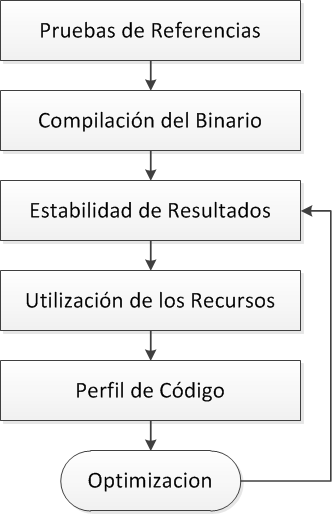
\includegraphics[width=5cm]{procedure.png}
\caption{Procedimiento de Análisis}
\end{figure}

\section{Paso a Paso}

A continuación se muestran los pasos a realizar, junto con preguntas que guían el análisis de rendimiento de una aplicación.

\subsection{Pruebas de Referencia}

\begin{enumerate}
\item Ejecutar pruebas de rendimiento sobre el sistema a utilizar para poder entender sus capacidades máximas en contraste con las teóricas.

\begin{lstlisting}
$ sudo apt-get install hpcc
$ mpirun -n `grep -c proc /proc/cpuinfo` ./hpcc
$ cat hpccoutf.txt
\end{lstlisting}

\begin{enumerate}
\item ¿Los resultados reflejan las capacidades esperadas del sistema?
\item ¿Los FLOPS se aproximan al rendimiento de un sistema similar?
\item ¿El rendimiento es $ CORES \times CLOCK \times FLOPS/CYCLE $ ?
\item ¿La latencia y ancho de banda de la memoria es la esperada?
\end{enumerate}

\item Comprobar variación de resultados para conocer la estabilidad de los mismos. La desviación estándar debe ser menor a 3 sigmas. Establecer cual es el promedio geométrico  a usar como referencia para comparaciones futuras.

\begin{lstlisting}
$ for i in `seq 1 32`; do /usr/bin/time -v ./app >> time.csv; done
\end{lstlisting}

\begin{enumerate}
\item ¿Son los resultados estables?
\item ¿La desviación estándar es menor que 3?
\item ¿Cuál es el promedio geométrico para comparaciones futuras?
\item ¿ Es necesario incrementar el problema para mejorar la desviación?
\item ¿ Es posible reducir el tiempo sin afectar la desviación?
\end{enumerate}

\item Escalar el problema para dimensionar la cantidad de trabajo según el tamaño del problema.

\begin{lstlisting}
$ for size in `seq 1024 1024 10240`; do /usr/bin/time -v ./app $size >> size.log; done
\end{lstlisting}

\begin{enumerate}
\item ¿Cuál es la relación entre el tiempo de las diferentes ejecuciones?
\item ¿Es la relación lineal o constante?
\end{enumerate}

\item Escalar cómputo para luego calcular límite de mejoras con {\it Amdalah} y {\it Gustafson}.

\begin{lstlisting}
$ for threads in `grep -c proc /proc/cpuinfo | xargs seq 1`; do OMP_NUM_THREADS=$threads ./app >> threads.log; done
\end{lstlisting}

\begin{enumerate}
\item ¿Cuál es la relación entre el tiempo de las diferentes ejecuciones?
\item ¿Es la relación lineal o constante?
\item ¿Qué porcentaje de la aplicación se estima paralelo?
\item ¿Cual es la mejora máxima posible?
\end{enumerate}

\item Generar el perfil de llamadas a funciones dentro de la aplicación para revisar el diseño de la misma y los posibles cuellos de botella a resolver.

\begin{lstlisting}
$ gcc -g -pg app.c -o app
$ ./app
\end{lstlisting}

\begin{lstlisting}
$ gprof --flat-profile --graph --annotated-source app
...
\end{lstlisting}

\begin{enumerate}
\item ¿Cómo esta diseñada la aplicación?
\item ¿Que dependencias en librerías externas tiene?
\item ¿Implementa algún núcleo de cómputo conocido encuadrado dentro de librerías optimizadas como BLAS?
\item ¿En que archivos, funciones y líneas se concentra la mayor cantidad de tiempo de cómputo?
\end{enumerate}

\item Utilizar el profiler a nivel de sistema

\begin{lstlisting}
$ prof stat ./app
$ prof record ./app
$ prof report
\end{lstlisting}

\begin{enumerate}
\item ¿Cómo se comporta el sistema durante la ejecución de la aplicación?
\item ¿Son las métricas de contadores de {\it hardware} las esperadas?
\item ¿Es la aplicación la gran concentradora de los recursos disponibles?
\item ¿Qué instrucciones de {\it hardware} son las utilizadas en el cuello de botella?
\end{enumerate}

\item Comprobar vectorizaciones

\begin{lstlisting}
$ gcc -Wall -Wextra -O3 --report-loop
\end{lstlisting}

\begin{enumerate}
\item ¿Hay ciclos que no pueden ser automáticamente vectorizados?
\end{enumerate}

\end{enumerate}

\chapter{Casos de Estudio}\label{chapter:cases}

Este capítulo aplica el procedimiento propuesto en el capítulo anterior. Varios ejemplos no triviales de aplicaciones de altas prestaciones son implementados y analizados utilizando los benchmarks y herramientas anteriormente presentadas.

\bigskip

La información de soporte sirve para realizar un análisis justificando potenciales optimizaciones con números y comportamiento cuantificado. Sin embargo como realizar una optimización no es trivial y depende del conocimiento de algoritmos que exploten adecuadamente la arquitectura del sistema.

\section{Rendimiento de Referencia}

El sistema utilizado es el mismo para todos los casos de prueba. A continuación se muestra su configuración de {\it hardware} y {\it software} (Tabla \ref{table:testbed}), además del resultado del rendimiento según HPCC con un proceso por core disponible.

\begin{table}[H]
    \caption{Hardware y software de cada nodo de cómputo}
    \centering
    \begin{tabular}{|l|l|}\hline
      {\bf Component} & {\bf Description} \\ \hline
      Placa Principal & Intel\textregistered 6 Series/C200 Series Chipset \\ \hline
      CPU & Intel\textregistered Xeon\textregistered CoreTM i7-2620M CPU @ 2.7GHz \\ \hline
      Controlador {\it Ethernet} & Intel\textregistered 82579V Gigabit Network \\ \hline
      Memoria RAM & 8 GB DDR3 \\ \hline
      Sistema Operativo & Ubuntu 10.02 LTS 64-bits \\ \hline
    \end{tabular}
    \label{table:testbed}
\end{table}

Una ejecución del benchmark HPCC nos muestra entonces el rendimiento a ser considerado como ideal en la práctica.

\label{table:pruebas}

\begin{verbatim}
HPL_Tflops=0.00701244
StarDGEMM_Gflops=2.21279
SingleDGEMM_Gflops=4.45068
PTRANS_GBs=0.661972
MPIRandomAccess_GUPs=0.000839626
StarRandomAccess_GUPs=0.0184879
SingleRandomAccess_GUPs=0.0359549
StarFFT_Gflops=1.11089
SingleFFT_Gflops=1.4984
MPIFFT_Gflops=2.42216
\end{verbatim}

\section{Multiplicación de Matrices}

La multiplicación de matrices es una operación fundamental en múltiples campos de aplicación científica como la resolución de ecuaciones lineales y la representación de grafos y espacios dimensionales. Por ello existe abundante material sobre el tema. Tomando como ejemplo una implementación utilizando OpenMP \footnote{\href{http://blog.speedgocomputing.com/2010/08/parallelizing-matrix-multiplication.html}{http://blog.speedgocomputing.com/2010/08/parallelizing-matrix-multiplication.html}.}, se procede a seguir la metodología propuesta en la sección anterior. 

\bigskip

Para una matriz de {\tt 2048} números de punto flotante de precisión simple, el promedio de ejecución tomó {\tt 2.036} segundos, la media geométrica {\tt 2.03567}. La desviación de resultados {\tt 0.03645}. Por lo tanto se puede concluir que es un buen conjunto de entrada para analizar rendimiento.

\bigskip

Al realizar ejecuciones con tamaños de entrada creciente los resultados fueron: {\tt N=1024 2.035678236} segundos, {\tt N=2048 18.853} segundos, {\tt N=3072 1m19.505} segundos y {\tt N=4096 3m42.779s} (Figura \ref{fig:matrix-problem}. 
Por defecto se ejecuta 1 {\it thread} por {\it core} disponible en el CPU.

\begin{figure}[H]
\centering
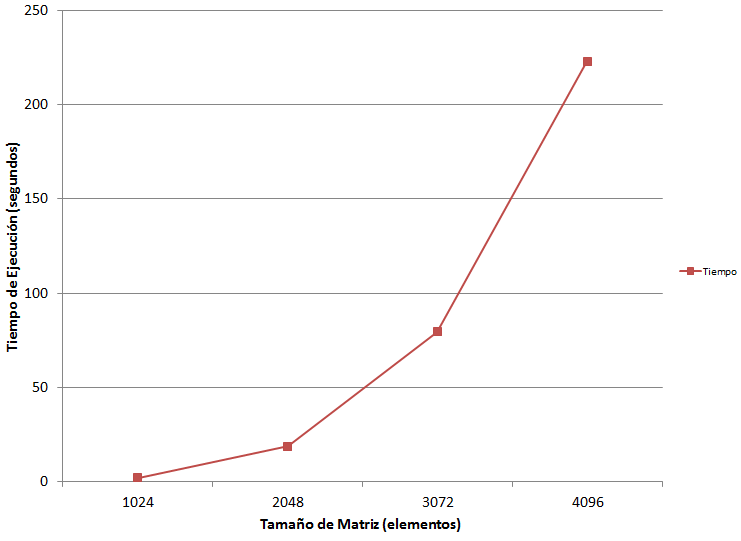
\includegraphics[width=\textwidth]{matrix-problem.png}
\caption{Tiempo de Ejecución con Diferentes Tamaños de Problema}
\label{fig:matrix-problem}
\end{figure}

Al realizar ejecuciones variando la cantidad de {\it threads} se obtuvieron los siguientes resultados (Figura \ref{fig:matrix-threads}). Calculamos entonces la proporción serial y paralela, 20\% y 80\% respectivamente. Los límites son entonces: {\it Amdalah} 5x y {\it Gustafson} 10x.

\begin{figure}[H]
\centering
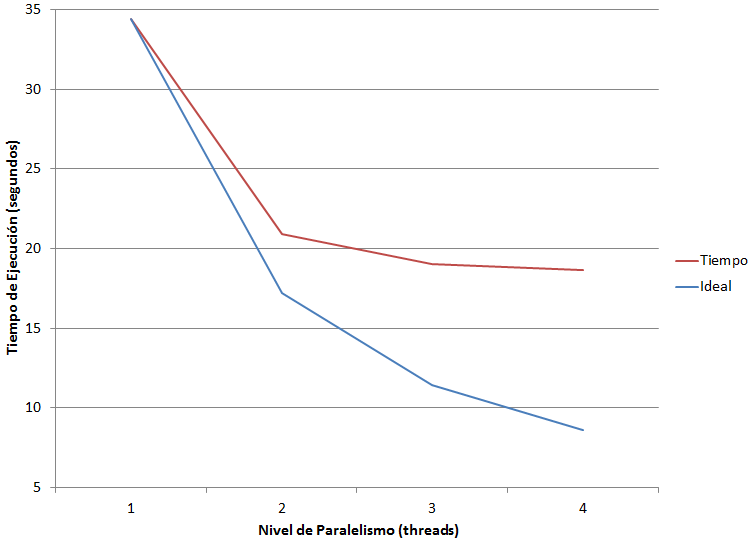
\includegraphics[width=10cm]{matrix-threads.png}
\caption{Tiempo de Ejecución con Diferente Número de Threads}
\label{fig:matrix-threads}
\end{figure}

Al aplicar las herramientas vistas previamente se identifica claramente que la multiplicación de los elementos de la matriz consume el mayor tiempo de cómputo. 

\begin{verbatim}
91.59% 111.61 main._omp_fn.0 (matrix.c:23)
6.56% 7.99 main._omp_fn.0 (matrix.c:22)
2.59% 3.16 main._omp_fn.0 (matrix.c:23)
\end{verbatim}

La gran mayoría del tiempo de ejecución del sistema se concentra en la aplicación.

\begin{verbatim}
97.43% matrix matrix [.] main._omp_fn.0
1.60% matrix [kernel.kallsyms] [k] __do_softirq
\end{verbatim}

El ciclo principal realiza la mayoría de las operaciones rápidamente, pero demora en la acumulación de resultados.

\begin{verbatim}
for (i = 0; i < SIZE; ++i) {
  for (j = 0; j < SIZE; ++j) {
    for (k = 0; k < SIZE; ++k) {
      c[i][j] += a[i][k] * b[k][j];
0.45 movaps %xmm2,%xmm0
0.03 movlps (%rax),%xmm0
0.07 movhps 0x8(%rax),%xmm0
1.35 add $0x4,%rax
0.24 shufps $0x0,%xmm0,%xmm0
0.04 mulps  (%rdx),%xmm0
81.36 add $0x2000,%rdx
\end{verbatim}

\begin{verbatim}
69278.383857 task-clock # 3.915 CPUs utilized
231 context-switches # 0.003 K/sec
4 CPU-migrations # 0.000 K/sec
12,461 page-faults # 0.180 K/sec
\end{verbatim}

Diferentes alternativas de implementación de esta operación son demostradas en \cite{mm-tool}, la 
Figura \ref{fig:mm} resume que utilizar una librería implementando BLAS es mejor que varios intentos de optimización.

\begin{figure}[H]
\centering
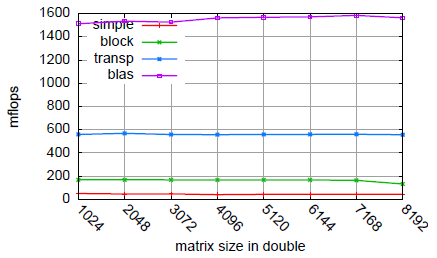
\includegraphics[width=10cm]{mm.png}
\caption{Comparación de Implementaciones}
\label{fig:mm}
\end{figure}

\section{Distribución de Calor en Dos Dimensiones}

Otro problema interesante es la simulación de transferencia de calor en un plano.
Se utiliza una grilla donde cada celda transfiere calor a sus vecinos en una serie de ciclos finitas simulando el paso del tiempo \footnote{\href{http://www.rblasch.org/studies/cs580/pa5/\#Source+Code-N100AC}{http://www.rblasch.org/studies/cs580/pa5/\#Source+Code-N100AC}.}.
Un gráfico de la salida del cálculo es mostrado en la Figura \ref{fig:heat}.

\begin{figure}[H]
\centering
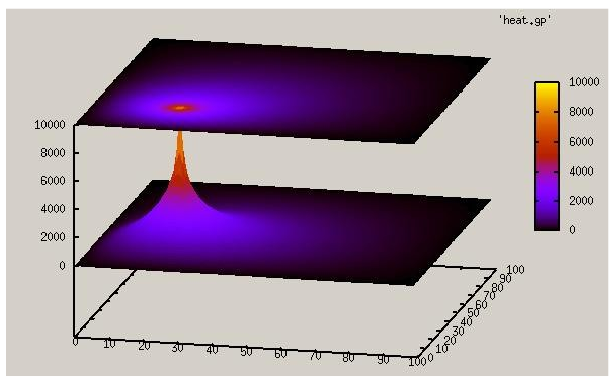
\includegraphics[width=10cm]{heat2d.png}
\caption{Simulación de Transferencia de Calor}
\label{fig:heat}
\end{figure}

Para un tamaño de matriz de {\tt N=300} números de punto flotante de precisión simple, el promedio de ejecución tomó {\tt 21.07913} segundos, la media geométrica {\tt 21.06550} segundos. La desviación de resultados fue de {\tt 0.76358}.
Por lo tanto se puede concluir que es un conjunto de datos de entrada estable.

\bigskip

Al realizar ejecuciones con tamaños de entrada creciente los resultados fueron:
{\tt N=300 21.0655}, {\tt N=400 40.31}, {\tt N=500 68.386}, {\tt N=600 118.213}, {\tt N=700 168.052} (Figura \ref{fig:heat-problem}).

\begin{figure}[H]
\centering
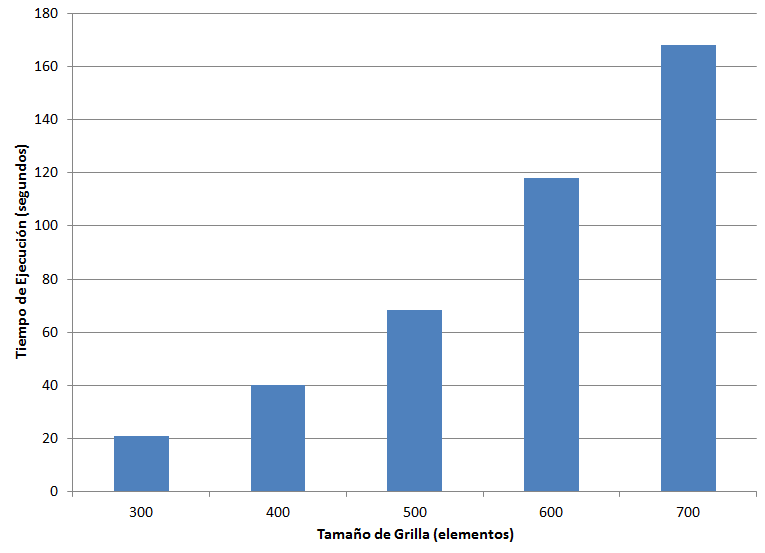
\includegraphics[width=10cm]{heat-problem.png}
\caption{Tiempo de Ejecución con Diferente Tamaño de Grilla}
\label{fig:heat-problem}
\end{figure}

\begin{figure}[H]
\centering
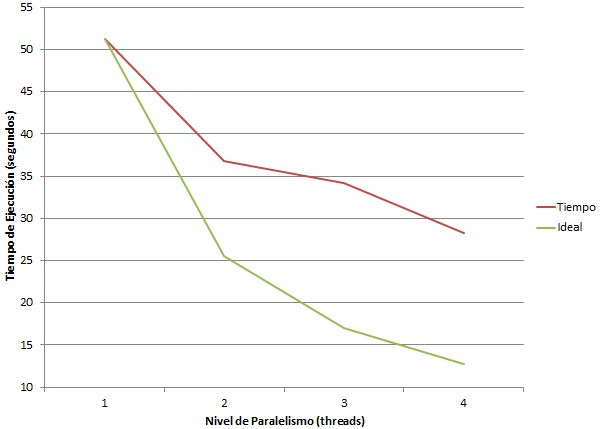
\includegraphics[width=10cm]{heat-threads.png}
\caption{Tiempo de Ejecución con Diferente Número de Threads}
\label{fig:heat-threads}
\end{figure}

Al realizar ejecuciones variando la cantidad de {\it threads} se obtuvieron los siguientes resultados (Figura \ref{fig:heat-threads}). Calculamos entonces la proporción serial y paralela, 20\% y 80\% respectivamente. Los límites son entonces: {\it Amdalah} $ 5 $ x y {\it Gustafson} $ 20 $ x.

\begin{verbatim}
109960.157161 task-clock # 3.839 CPUs utilized
2,244 context-switches # 0.020 K/sec
6 CPU-migrations # 0.000 K/sec
1,160 page-faults # 0.011 K/sec
\end{verbatim}

Un perfil del sistema nos localiza el computo en nuestro núcleo de computación, seguida del maneja de threads por parte de la implementación GNU de OpenMP.

\begin{verbatim}
78.38% heat heat [.] compute_one_iteration._omp_fn.0
20.61% heat libgomp.so.1.0.0 [.] 0x00000000000093be
\end{verbatim}

Un perfil de la aplicación nos demuestra que el 35.05\% del tiempo de ejecución se concentra en la línea que realiza el promedio de las celdas vecinas. Y casi el 13.79\% donde se ajusta el promedio por la diferencia de temperatura por ciclo.

\begin{verbatim}
35.05% 28.71 compute_one_iteration._omp_fn.0 (heat.c:77)
13.79% 11.30 compute_one_iteration._omp_fn.0 (heat.c:82)
\end{verbatim}

Un nivel más detallado nos muestra específicamente que instrucciones del procesador están en juego.

\begin{verbatim}
#pragma omp parallel for shared(solution,cur_gen,next_gen,diff_constant) private(i,j)
for (i = 1; i <= RESN; i++)
  for (j = 1; j <= RESN; j++)
    solution[next_gen][i][j] = solution[cur_gen][i][j] +
 21.79 addpd  %xmm1,%xmm0
 15.13 movlpd %xmm0,(%rdx,%rax,1)
  2.94 movhpd %xmm0,0x8(%rdx,%rax,1)
  5.66 add $0x10,%rax
\end{verbatim}

\section{Problema de las Ocho Reinas}

El dilema trata en el problema de posicionar en un tablero de ajedrez ocho
reinas sin que alguna amenace a las demás. Una reina amenaza a cualquier otra
pieza en el tablero que este en la mismo diagonal, fila o columna.

\bigskip

El problema de encontrar todas las soluciones para un tamaño de tablero dado suele resolverse utilizando recursión \footnote{\href{http://www.stevenpigeon.org/blogs/hbfs/super-reines-openmp.cpp}{http://www.stevenpigeon.org/blogs/hbfs/super-reines-openmp.cpp}.}.

\begin{figure}[H]
\centering
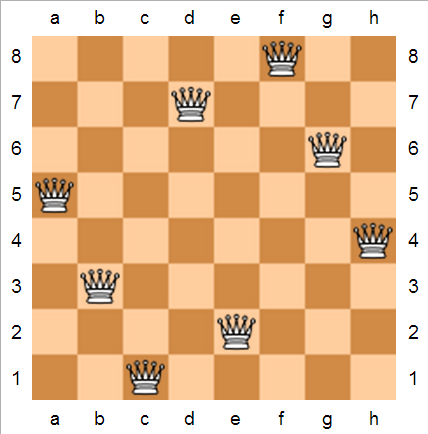
\includegraphics[width=7cm]{queen.png}
\caption{Solución simétrica del problema de las 8 reinas [Wikipedia]}
\end{figure}

Ejercitando el problema con {\tt N=16} nos da un promedio de ejecución de {\tt 31.39727} segundos, y una media geométrica de {\tt 31.39346} segundos. Con una desviación de resultado de {\tt 0.5102}. Podemos concluir que los resultados son estables.

\bigskip

El escalamiento de tamaño y cantidad de unidades de cómputo refleja un comportamiento no deseado.

\begin{figure}[H]
\centering
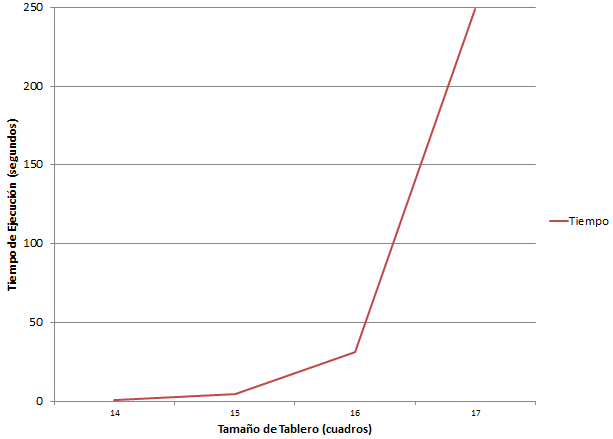
\includegraphics[width=10cm]{queen-problem.png}
\caption{Tiempo de Ejecución con Diferente Tamaño de Tablero}
\label{fig:queen-problem}
\end{figure}

\begin{figure}[H]
\centering
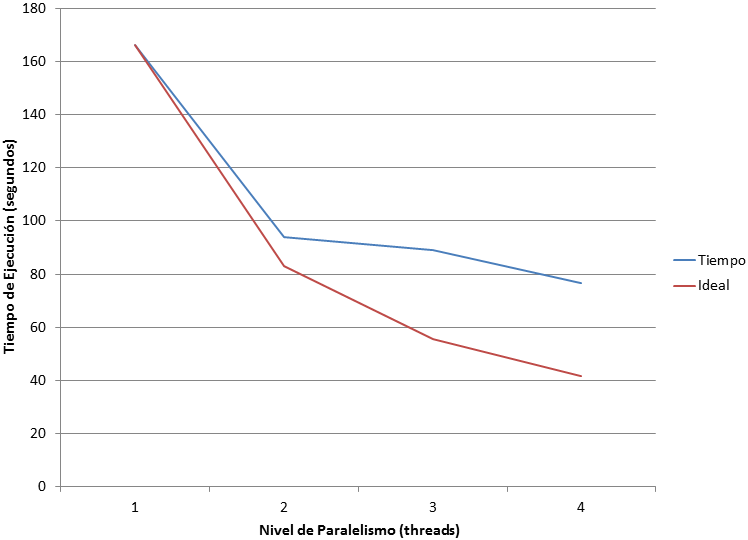
\includegraphics[width=10cm]{queen-scaling.png}
\caption{Tiempo de Ejecución con Diferente Tamaño de Tablero}
\label{fig:queen-scaling}
\end{figure}

\begin{verbatim}
302506.712420 task-clock                #    3.610 CPUs utilized
               545 context-switches          #    0.002 K/sec
                 3 CPU-migrations            #    0.000 K/sec
               382 page-faults               #    0.001 K/sec
\end{verbatim}

Un perfil del sistema muestra un uso casi totalitario por parte de la aplicación.

\begin{verbatim}
97.64% queens queens [.] solve(int, int, unsigned long,
  unsigned long, unsigned long)
1.56% queens [kernel.kallsyms] [k] __do_softirq
\end{verbatim}

Un perfil de la aplicación muestra que el cuello de botella se encuentra en la determinación de amenazas por parte de
otras reinas.

\begin{verbatim}
21.95 19.73 test (queens.cc:51)
12.81 11.52 test (queens.cc:51)
8.72 7.84 test (queens.cc:51)
\end{verbatim}

Un detalle de la operación muestra el tiempo que toma cada instrucción.

\begin{verbatim}
solve(int, int, unsigned long, unsigned long, unsigned long,
  uint64_t diag135, uint64_t cols)                                                                                             {
10.86 lea (%rdx,%r11,1),%ecx
{
  return ((cols & (1ull << j))
    + (diag135 & (1ull << (j+k)))
    + (diag45 & (1ull << (32+j-k))))==0;
0.85 mov %r14,%rdx
1.49 mov %rax,%rsi
2.95 shl %cl,%rdx
9.81 mov %r8,%rcx
1.15 and %rbp,%rsi
2.17 and %r12,%rcx
2.06 add %rsi,%rcx
4.73 mov %rdx,%rsi
1.49 and %r13,%rsi
\end{verbatim}

\chapter{Conclusiones}\label{chapter:conclusions}

La optimización del rendimiento de una aplicación es algo no trivial.
Es preciso realizar un análisis disciplinado del comportamiento y del uso de los recursos antes de
empezar a optimizar. Las mejoras pueden ser no significativas si son realizadas en el lugar incorrecto.

\bigskip

Este trabajo soporta los primeros pasos de análisis de rendimiento para expertos del dominio de un problema científico utilizando computación de altas prestaciones. Se provee una metodología de uso de herramientas de soporte para principiantes, que puede ser utilizada como una lista de pasos resumidos para usuarios casuales, e incluso como referencia de consulta diaria para expertos.

\bigskip

Se resume también el estado del arte del análisis de rendimiento en
aplicaciones de cómputo de altas prestaciones. Respecto a herramientas de soporte, se detallan
diferentes opciones y se demuestra su aplicación en varios problemas simples aunque suficientemente interesantes. 
Este estudio propone un proceso de análisis de rendimiento gradual e iterativo que
puede ser tomado como trabajo previo de una implementación práctica del mismo. Es decir
incluyendo soporte automático para la aplicación de las herramientas y la generación integrada de
reportes de rendimiento. La utilización de estas ideas en una aplicación del mundo real es materia
pendiente, otra posibilidad es re-implementar desde cero alguna aplicación
científica en colaboración con algún grupo de investigación y realizar
varios ciclos de optimización para validar su utilidad.

\bibliography{report}

\end{document}
